\documentclass{article}

\usepackage[a3paper, landscape, margin=.5cm]{geometry}

\usepackage{tikz}

\begin{document}

\begin{tikzpicture}[scale = 1]
  \def\base{2cm}
  \def\framethickness{.01cm}
  \def\rulethickness{.1cm}
  \def\ruleheight{.9cm}
  \def\ruleticsheight{.3cm}
  \def\ruleticksnb{19}

  \draw[line width=\framethickness]
      (0,0) rectangle (\ruleticksnb*\base+\base,\ruleheight);

  \foreach \i in {1,...,\ruleticksnb}
  {
    \draw[color=black,line width=\rulethickness]%
        (\i*\base,\ruleheight-\ruleticsheight) -- (\i*\base,\ruleheight)%
        node[anchor=north,yshift=-\ruleticsheight] {\Large \textbf{\i}};
  }

  \draw[line width=\rulethickness]
      (0cm,\ruleheight-.5*\rulethickness) -- coordinate (x axis mid)
      (\ruleticksnb*\base+\base,\ruleheight-.5*\rulethickness);
\end{tikzpicture}

\end{document}
